% !TEX root = ../thesis.tex

\def\lafigsize{.491\linewidth}
\def\lafigdesc{Visualization of outputs created by the \la based on an example data set of the Sparkling Lake, WI, USA}
\begin{figure}[!htb]
  \centering
  \begin{subfigure}{\lafigsize}
    \caption{\label{fig:la:out:Ln}Lake Number}
    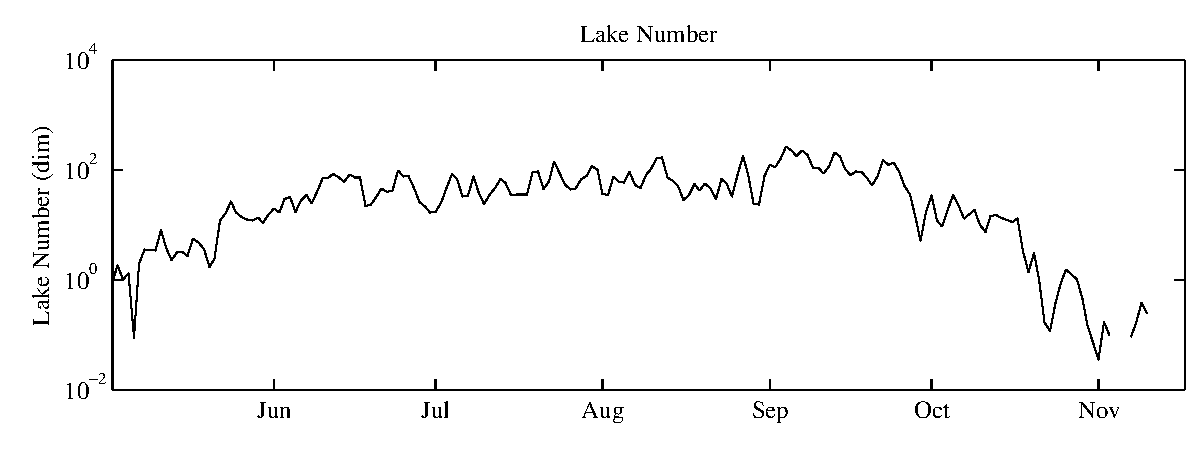
\includegraphics[width = \linewidth]{figures/Sparkling_Ln.pdf}
  \end{subfigure}
  \begin{subfigure}{\lafigsize}
    \caption{\label{fig:la:out:SLn}Seasonal Lake Number}
    \includegraphics[width = \linewidth]{figures/Sparkling_SLn.pdf}
  \end{subfigure}
  \begin{subfigure}{\lafigsize}
    \caption{\label{fig:la:out:metaT}Metalimnion Top}
    \includegraphics[width = \linewidth]{figures/Sparkling_metaT.pdf}
  \end{subfigure}
  \begin{subfigure}{\lafigsize}
    \caption{\label{fig:la:out:metaB}Metalimnion Bottom}
    \includegraphics[width = \linewidth]{figures/Sparkling_metaB.pdf}
  \end{subfigure}
  \begin{subfigure}{\lafigsize}
    \caption{\label{fig:la:out:SmetaT}Seasonal Metalimnion Top}
    \includegraphics[width = \linewidth]{figures/Sparkling_SmetaT.pdf}
  \end{subfigure}
  \begin{subfigure}{\lafigsize}
    \caption{\label{fig:la:out:SmetaB}Seasonal Metalimnion Bottom}
    \includegraphics[width = \linewidth]{figures/Sparkling_SmetaB.pdf}
  \end{subfigure}
  \begin{subfigure}{\lafigsize}
    \caption{\label{fig:la:out:N2}Buoyancy Frequency}
    \includegraphics[width = \linewidth]{figures/Sparkling_N2.pdf}
  \end{subfigure}
  \begin{subfigure}{\lafigsize}
    \caption{\label{fig:la:out:SN2}Seasonal Buoyancy Frequency}
    \includegraphics[width = \linewidth]{figures/Sparkling_SN2.pdf}
  \end{subfigure}
  \begin{subfigure}{\lafigsize}
    \caption{\label{fig:la:out:T1}Mode-1 Vertical Seiche Period}
    \includegraphics[width = \linewidth]{figures/Sparkling_T1.pdf}
  \end{subfigure}
  \begin{subfigure}{\lafigsize}
    \caption{\label{fig:la:out:ST1}Seasonal Mode-1 Vertical Seiche Period}
    \includegraphics[width = \linewidth]{figures/Sparkling_ST1.pdf}
  \end{subfigure}
  \caption[\lafigdesc.]{\label{fig:la:outputs:1}\lafigdesc{} \emph{(continued on \cpageref{fig:la:outputs:2})}.}
\end{figure}
\begin{figure}
  \ContinuedFloat\centering\captionsetup{list=no}
  \begin{subfigure}{\lafigsize}
    \caption{\label{fig:la:out:W}Wedderburn Number}
    \includegraphics[width = \linewidth]{figures/Sparkling_W.pdf}
  \end{subfigure}
  \begin{subfigure}{\lafigsize}
    \caption{\label{fig:la:out:SW}Seasonal Wedderburn Number}
    \includegraphics[width = \linewidth]{figures/Sparkling_SW.pdf}
  \end{subfigure}
  \begin{subfigure}{\lafigsize}
    \caption{\label{fig:la:out:thermD}Thermocline Depth}
    \includegraphics[width = \linewidth]{figures/Sparkling_thermD.pdf}
  \end{subfigure}
  \begin{subfigure}{\lafigsize}
    \caption{\label{fig:la:out:SthermD}Seasonal Thermocline Depth}
    \includegraphics[width = \linewidth]{figures/Sparkling_SthermD.pdf}
  \end{subfigure}
  \begin{subfigure}{\lafigsize}
    \caption{\label{fig:la:out:uSt}$u^{*}$}
    \includegraphics[width = \linewidth]{figures/Sparkling_uSt.pdf}
  \end{subfigure}
  \begin{subfigure}{\lafigsize}
    \caption{\label{fig:la:out:SuSt}Seasonal $u^{*}$}
    \includegraphics[width = \linewidth]{figures/Sparkling_SuSt.pdf}
  \end{subfigure}
  \begin{subfigure}{\lafigsize}
    \caption{\label{fig:la:out:St}Schmidt Stability}
    \includegraphics[width = \linewidth]{figures/Sparkling_St.pdf}
  \end{subfigure}
  \begin{subfigure}{\lafigsize}
    \caption{\label{fig:la:out:wndSpd}Wind Speed}
    \includegraphics[width = \linewidth]{figures/Sparkling_wndSpd.pdf}
  \end{subfigure}
  \begin{subfigure}{\lafigsize}
    \caption{\label{fig:la:out:wTemp}Water Temperature}
    \includegraphics[width = \linewidth]{figures/Sparkling_wTemp.pdf}
  \end{subfigure}
  \caption{\label{fig:la:outputs:2}\lafigdesc.}
\end{figure}
